%!TEX root = ../../report.tex
\section{Costmap for path planning}
The path planning not only uses the lethal obstacles but also considers less costly cells in order to determine the best path. Therefore the dynamic obstacle should be represented in some way to help guide the path planning away from obstacles that might obstruct the path, possibly cause a re-planning to be necessary. Because path planning is most likely handled without observing most of the path certain predictions will have to be made regarding the cost of each cell. The Markov model used in the dynamic map is well suited to estimate the probability distribution between the possible states, in this case free or occupied. 
As the time of the last observation also is logged it is possible to calculate to number of steps the Markov chain must go through to project the state to the current time. Using the last observation as the initial distribution, the chain can easily be calculated. One issue with this is the possibility of an uncertain observation. If an observation is very uncertain, thus close to 0.5, it carries very little information and therefore not very suitable to be used in the forward projection. As it is not desirable to use uncertain values as basis for the forward projection, an update and predict system is used. Each time a new value is received the current occupied probability estimate, \(p_{occ\_est}(i)\), is updated as shown in equation \ref{eq:cost_update}.

\begin{equation}
\label{eq:cost_update}
p_{occ\_est}(i) = p_{occ\_est}(i-1) +  2 \cdot |p_{occ\_meas} - 0.5| \cdot (p_{occ\_meas} - p_{occ\_est}(i-1))
\end{equation}

In equation \ref{eq:cost_update} the term  \(2 \cdot |p_{occ\_meas} -0.5|\) is the state score used in the PMAC learner. The state score here is used to weight the new measurement in the update. Figure \ref{fig:cost_update} shows an example of the update method for the \(p_{occ\_est}\). The weight values are shown with sign to indicate if the weight is towards occupied or free. 

\begin{figure}[htbp]
	\centering
	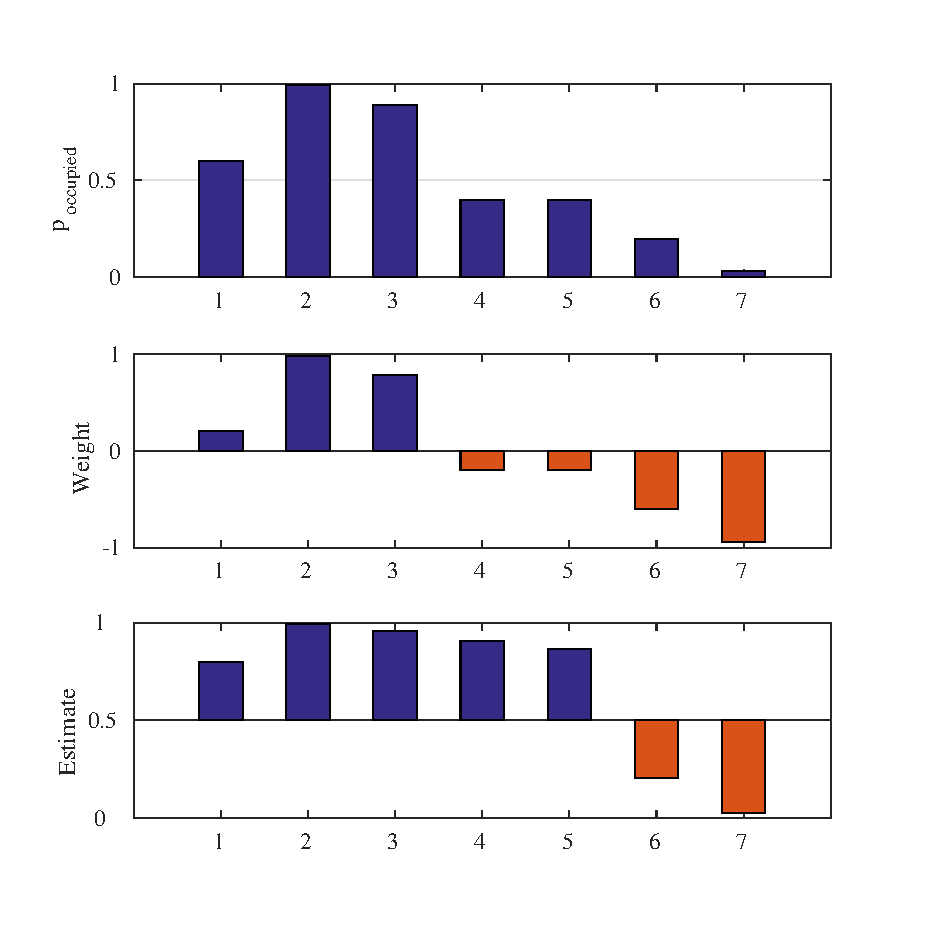
\includegraphics[width=1\linewidth]{chapters/cost_interpretation/figures/update}
	\caption{Update of the estimated occupancy. Sign in weight indicates free or occupied, positive is occupied. }
	\label{fig:cost_update}
\end{figure}

It is seen in figure \ref{fig:cost_update} that uncertain free values does not cause a great shift in the estimated occupancy value. When the free observations become increasingly certain a significant change is observed. 

The predict steps are performed when a new map is to be generated. At this time all cells are projected forward from their last observed time to the current time. This is done by using the estimated occupancy as the initial distribution and then projecting forward a number of steps according to the time difference between last observation and the current time. If the number of steps projected is large, then the estimate is not used. Instead the stationary distribution in  equation \ref{eq:long_term}  determines the final occupancy probability [REF HMM].
\begin{equation}
	\label{eq:long_term}
	p_{stationary} = \frac{1}{\lambda_{entry} + \lambda_{exit}} \cdot \lambda_{entry}
\end{equation}

Figure \ref{fig:cost_predict} shows the projection of a cell with the Markov parameters \(\lambda_{exit} = 0.13 \) and \(\lambda_{entry} = 0.52 \). The initial probability estimate is the final estimate form figure \ref{fig:cost_update}. The red dotted line shows the result of the long term calculation. It is clear that in this case, it does not take many forward projection until it converges close to the long term. The predicted occupancy is then scaled into the proper value range for the subscribing systems to use. 

\begin{figure}[htbp]
	\centering
	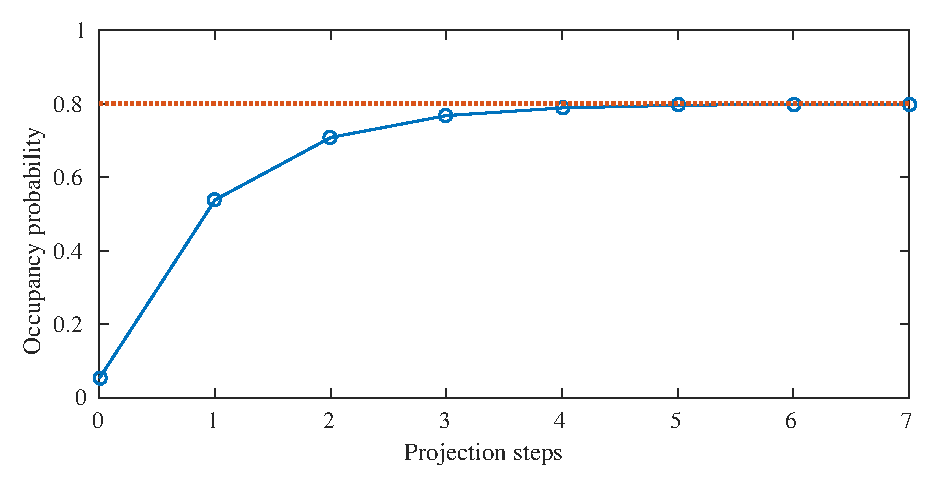
\includegraphics[width=1\linewidth]{chapters/cost_interpretation/figures/projection}
	\caption{Prediction of occupancy. Markov parameters: \(\lambda_{entry} = 0.52\), \(\lambda_{exit} = 0.13\)}
	\label{fig:cost_predict}
\end{figure}